\documentclass[]{ctexbook}
\usepackage{lmodern}
\usepackage{amssymb,amsmath}
\usepackage{ifxetex,ifluatex}
\usepackage{fixltx2e} % provides \textsubscript
\ifnum 0\ifxetex 1\fi\ifluatex 1\fi=0 % if pdftex
  \usepackage[T1]{fontenc}
  \usepackage[utf8]{inputenc}
\else % if luatex or xelatex
  \ifxetex
    \usepackage{xltxtra,xunicode}
  \else
    \usepackage{fontspec}
  \fi
  \defaultfontfeatures{Ligatures=TeX,Scale=MatchLowercase}
\fi
% use upquote if available, for straight quotes in verbatim environments
\IfFileExists{upquote.sty}{\usepackage{upquote}}{}
% use microtype if available
\IfFileExists{microtype.sty}{%
\usepackage{microtype}
\UseMicrotypeSet[protrusion]{basicmath} % disable protrusion for tt fonts
}{}
\usepackage[b5paper,tmargin=2.5cm,bmargin=2.5cm,lmargin=3.5cm,rmargin=2.5cm]{geometry}
\usepackage[unicode=true]{hyperref}
\PassOptionsToPackage{usenames,dvipsnames}{color} % color is loaded by hyperref
\hypersetup{
            pdftitle={计算机时代统计推断},
            pdfauthor={张晨阳},
            colorlinks=true,
            linkcolor=Maroon,
            citecolor=Blue,
            urlcolor=Blue,
            breaklinks=true}
\urlstyle{same}  % don't use monospace font for urls
\usepackage{natbib}
\bibliographystyle{apalike}
\usepackage{color}
\usepackage{fancyvrb}
\newcommand{\VerbBar}{|}
\newcommand{\VERB}{\Verb[commandchars=\\\{\}]}
\DefineVerbatimEnvironment{Highlighting}{Verbatim}{commandchars=\\\{\}}
% Add ',fontsize=\small' for more characters per line
\usepackage{framed}
\definecolor{shadecolor}{RGB}{248,248,248}
\newenvironment{Shaded}{\begin{snugshade}}{\end{snugshade}}
\newcommand{\AlertTok}[1]{\textcolor[rgb]{0.94,0.16,0.16}{#1}}
\newcommand{\AnnotationTok}[1]{\textcolor[rgb]{0.56,0.35,0.01}{\textbf{\textit{#1}}}}
\newcommand{\AttributeTok}[1]{\textcolor[rgb]{0.77,0.63,0.00}{#1}}
\newcommand{\BaseNTok}[1]{\textcolor[rgb]{0.00,0.00,0.81}{#1}}
\newcommand{\BuiltInTok}[1]{#1}
\newcommand{\CharTok}[1]{\textcolor[rgb]{0.31,0.60,0.02}{#1}}
\newcommand{\CommentTok}[1]{\textcolor[rgb]{0.56,0.35,0.01}{\textit{#1}}}
\newcommand{\CommentVarTok}[1]{\textcolor[rgb]{0.56,0.35,0.01}{\textbf{\textit{#1}}}}
\newcommand{\ConstantTok}[1]{\textcolor[rgb]{0.00,0.00,0.00}{#1}}
\newcommand{\ControlFlowTok}[1]{\textcolor[rgb]{0.13,0.29,0.53}{\textbf{#1}}}
\newcommand{\DataTypeTok}[1]{\textcolor[rgb]{0.13,0.29,0.53}{#1}}
\newcommand{\DecValTok}[1]{\textcolor[rgb]{0.00,0.00,0.81}{#1}}
\newcommand{\DocumentationTok}[1]{\textcolor[rgb]{0.56,0.35,0.01}{\textbf{\textit{#1}}}}
\newcommand{\ErrorTok}[1]{\textcolor[rgb]{0.64,0.00,0.00}{\textbf{#1}}}
\newcommand{\ExtensionTok}[1]{#1}
\newcommand{\FloatTok}[1]{\textcolor[rgb]{0.00,0.00,0.81}{#1}}
\newcommand{\FunctionTok}[1]{\textcolor[rgb]{0.00,0.00,0.00}{#1}}
\newcommand{\ImportTok}[1]{#1}
\newcommand{\InformationTok}[1]{\textcolor[rgb]{0.56,0.35,0.01}{\textbf{\textit{#1}}}}
\newcommand{\KeywordTok}[1]{\textcolor[rgb]{0.13,0.29,0.53}{\textbf{#1}}}
\newcommand{\NormalTok}[1]{#1}
\newcommand{\OperatorTok}[1]{\textcolor[rgb]{0.81,0.36,0.00}{\textbf{#1}}}
\newcommand{\OtherTok}[1]{\textcolor[rgb]{0.56,0.35,0.01}{#1}}
\newcommand{\PreprocessorTok}[1]{\textcolor[rgb]{0.56,0.35,0.01}{\textit{#1}}}
\newcommand{\RegionMarkerTok}[1]{#1}
\newcommand{\SpecialCharTok}[1]{\textcolor[rgb]{0.00,0.00,0.00}{#1}}
\newcommand{\SpecialStringTok}[1]{\textcolor[rgb]{0.31,0.60,0.02}{#1}}
\newcommand{\StringTok}[1]{\textcolor[rgb]{0.31,0.60,0.02}{#1}}
\newcommand{\VariableTok}[1]{\textcolor[rgb]{0.00,0.00,0.00}{#1}}
\newcommand{\VerbatimStringTok}[1]{\textcolor[rgb]{0.31,0.60,0.02}{#1}}
\newcommand{\WarningTok}[1]{\textcolor[rgb]{0.56,0.35,0.01}{\textbf{\textit{#1}}}}
\usepackage{longtable,booktabs}
% Fix footnotes in tables (requires footnote package)
\IfFileExists{footnote.sty}{\usepackage{footnote}\makesavenoteenv{long table}}{}
\IfFileExists{parskip.sty}{%
\usepackage{parskip}
}{% else
\setlength{\parindent}{0pt}
\setlength{\parskip}{6pt plus 2pt minus 1pt}
}
\setlength{\emergencystretch}{3em}  % prevent overfull lines
\providecommand{\tightlist}{%
  \setlength{\itemsep}{0pt}\setlength{\parskip}{0pt}}
\setcounter{secnumdepth}{5}
% Redefines (sub)paragraphs to behave more like sections
\ifx\paragraph\undefined\else
\let\oldparagraph\paragraph
\renewcommand{\paragraph}[1]{\oldparagraph{#1}\mbox{}}
\fi
\ifx\subparagraph\undefined\else
\let\oldsubparagraph\subparagraph
\renewcommand{\subparagraph}[1]{\oldsubparagraph{#1}\mbox{}}
\fi

% set default figure placement to htbp
\makeatletter
\def\fps@figure{htbp}
\makeatother

\usepackage{booktabs}
\usepackage{longtable}

\usepackage{framed,color}
\definecolor{shadecolor}{RGB}{248,248,248}

\renewcommand{\textfraction}{0.05}
\renewcommand{\topfraction}{0.8}
\renewcommand{\bottomfraction}{0.8}
\renewcommand{\floatpagefraction}{0.75}

\let\oldhref\href
\renewcommand{\href}[2]{#2\footnote{\url{#1}}}

\makeatletter
\newenvironment{kframe}{%
\medskip{}
\setlength{\fboxsep}{.8em}
 \def\at@end@of@kframe{}%
 \ifinner\ifhmode%
  \def\at@end@of@kframe{\end{minipage}}%
  \begin{minipage}{\columnwidth}%
 \fi\fi%
 \def\FrameCommand##1{\hskip\@totalleftmargin \hskip-\fboxsep
 \colorbox{shadecolor}{##1}\hskip-\fboxsep
     % There is no \\@totalrightmargin, so:
     \hskip-\linewidth \hskip-\@totalleftmargin \hskip\columnwidth}%
 \MakeFramed {\advance\hsize-\width
   \@totalleftmargin\z@ \linewidth\hsize
   \@setminipage}}%
 {\par\unskip\endMakeFramed%
 \at@end@of@kframe}
\makeatother

\makeatletter
\@ifundefined{Shaded}{
}{\renewenvironment{Shaded}{\begin{kframe}}{\end{kframe}}}
\@ifpackageloaded{fanyverb}{%
  % https://github.com/CTeX-org/ctex-kit/issues/331
  \RecustomVerbatimEnvironment{Highlighting}{Verbatim}{commandchars=\\\{\},formatcom=\xeCJKVerbAddon}%
}{}
\makeatother

\usepackage{makeidx}
\makeindex

\urlstyle{tt}

\usepackage{amsthm}
\makeatletter
\def\thm@space@setup{%
  \thm@preskip=8pt plus 2pt minus 4pt
  \thm@postskip=\thm@preskip
}
\makeatother

\frontmatter

\title{计算机时代统计推断}
\author{张晨阳}
\date{2018-08-02}

\usepackage{amsthm}
\newtheorem{theorem}{Theorem}[chapter]
\newtheorem{lemma}{Lemma}[chapter]
\theoremstyle{definition}
\newtheorem{definition}{Definition}[chapter]
\newtheorem{corollary}{Corollary}[chapter]
\newtheorem{proposition}{Proposition}[chapter]
\theoremstyle{definition}
\newtheorem{example}{Example}[chapter]
\theoremstyle{definition}
\newtheorem{exercise}{Exercise}[chapter]
\theoremstyle{remark}
\newtheorem*{remark}{Remark}
\newtheorem*{solution}{Solution}
\let\BeginKnitrBlock\begin \let\EndKnitrBlock\end
\begin{document}
\maketitle


\thispagestyle{empty}

\begin{center}
献给……

呃,爱谁谁吧
\end{center}

\setlength{\abovedisplayskip}{-5pt}
\setlength{\abovedisplayshortskip}{-5pt}

{
\setcounter{tocdepth}{2}
\tableofcontents
}
\listoftables
\listoffigures
\chapter*{前言}


你好,世界。我写了一本书。这本书是这样的,第 \ref{intro}
章介绍了啥啥,第 \ref{wind} 章说了啥啥,然后是啥啥\ldots{}\ldots{}

我用了两个 R 包编译这本书,分别是 \textbf{knitr}\index{knitr}
\citep{xie2015} 和 \textbf{bookdown}\index{bookdown}
\citep{R-bookdown}。以下是我的 R 进程信息:

\begin{Shaded}
\begin{Highlighting}[]
\KeywordTok{sessionInfo}\NormalTok{()}
\end{Highlighting}
\end{Shaded}

\begin{verbatim}
## R version 3.5.0 (2018-04-23)
## Platform: x86_64-apple-darwin15.6.0 (64-bit)
## Running under: macOS High Sierra 10.13
## 
## Matrix products: default
## BLAS: /Library/Frameworks/R.framework/Versions/3.5/Resources/lib/libRblas.0.dylib
## LAPACK: /Library/Frameworks/R.framework/Versions/3.5/Resources/lib/libRlapack.dylib
## 
## locale:
## [1] en_US.UTF-8/en_US.UTF-8/en_US.UTF-8/C/en_US.UTF-8/en_US.UTF-8
## 
## attached base packages:
## [1] stats     graphics  grDevices utils     datasets 
## [6] methods   base     
## 
## loaded via a namespace (and not attached):
##  [1] Rcpp_0.12.17    bookdown_0.7    digest_0.6.15  
##  [4] rprojroot_1.3-2 backports_1.1.2 magrittr_1.5   
##  [7] evaluate_0.10.1 highr_0.7       stringi_1.2.3  
## [10] rstudioapi_0.7  rmarkdown_1.10  tools_3.5.0    
## [13] stringr_1.3.1   xfun_0.3        yaml_2.1.19    
## [16] compiler_3.5.0  htmltools_0.3.6 knitr_1.20
\end{verbatim}

\section*{致谢}


非常感谢谁谁以及谁谁对我的帮助。艾玛,要不是他们神一样的队友,我两年前就写完这本书了。

\BeginKnitrBlock{flushright}
张三\\
于 A 村某角落
\EndKnitrBlock{flushright}

\hypertarget{author}{%
\chapter*{作者简介}\label{author}}


上不了厅堂,下得了厨房。敲得了代码,逮得住蟑螂。

\mainmatter

\hypertarget{intro}{%
\chapter{算法和推断 Algorithms and Inference}\label{intro}}

Statistics is the science of learning from experience, particularly
experience that arrives a little bit at a time: the successes and
failures of a new experimental drug, the uncertain measurements of an
asteroid's path to-ward Earth. It may seem surprising that any one
theory can cover such an amorphous target as ``learning from
experience.'' In fact, there are \emph{two} main statistical theories.
Bayesianism and frequentism, whose connections and disagreements animate
many of the succeeding chapters.

统计学是一个从经验中学习的学科,尤其是\emph{每次得到一点点的经验}:一种新型试验药的成功与失败,小行星驶向地球路径的不确定性测量。任何一个理论都能\emph{适用}这样一个模糊的目标:``从经验中学习'',这似乎令人惊讶。事实上,有两种主要的统计理论。贝叶斯主义和频率派,它们的联系和分歧推动了许多后续章节。

First, however, we want to discuss a less philosophical, more
operational division of labor that applies to both theories: between the
\emph{algorithmic} and \emph{inferential} aspects of statistical method,
averaging. Suppose we have observed numbers
\(x _ { 1 } , x _ { 2 } , \dots . . . x _ { n }\)applying to some
phenomenon of interest, perhaps the automobile accident rates in the n =
50 states. The \emph{mean}

\[
\overline { x } = \sum _ { i = 1 } ^ { n } x _ { i } / n
\]

然而,首先,我们要讨论适用于两种理论的较少哲学,更具操作性的分工:统计方法的算法和推断方面之间的平均。假设我们观察到某些我们感兴趣的数:
\(x _ { 1 } , x _ { 2 } , \dots . . . x _ { n }\),就当是 50
个州汽车事故率,它们的均值是:

\[
\overline { x } = \sum _ { i = 1 } ^ { n } x _ { i } / n
\]

Summarizse the result in a single number.

将结果汇总到一个数值中。

How accurate is that number? The textbook answer is given in terms of
the \emph{standard error},

那么得到数值的准确度是多少呢?教科书给出的答案是\emph{标准误},

\[
\hat { s e } = \left[ \sum _ { i = 1 } ^ { n } \left( x _ { i } - \overline { x } \right) ^ { 2 } / ( n ( n - 1 ) ) \right] ^ { 1 / 2 }
\]

Here \emph{averaging(1)} is the algorithm, while the standard error
provides an inference of algorithm's accuracy . It is a crucial, aspect
of the statistical theory that same data that supplied an estimate can
also assess its accuracy.\footnote{``Inference'' concerns more than
  accuracy: speaking broardly, algorithms say what the statistician does
  while inference says why he or she does it. -
  ``推断''不仅仅关注准确性:从广义上讲,算法说明统计学家所做的事情,而推理则说明为什么他或她这样做。}

这里平均(1)是算法,而标准误差提供算法精度的推断。
统计理论的一个重要方面是,用于估计的数据也可以评估估计的准确性。

Of course, \(\hat{se}\)(3) is itself an algorithm, which could be (and
is) subject to further inferential analysis concerning \emph{its}
accuracy. The point is that the algorithm come first and the inference
follows at the second level of statistical consideration. In practice
this means that algorithm invention is a more free-wheeling and
adventurous enterprise, with inference playing catch-up as it strives to
assess the accuracy, good or bad, of some hot new algorithmic
methodology.

当然,\(\hat{se}\)本身就是一种算法,它可以(而且是)对其准确性进行进一步的推论分析。
关键是算法首先出现,\emph{推断遵循统计考虑的第二个层次}。
在实践中,这意味着算法发明是一个更加自由和冒险的事业,当它努力评估一些热门的新算法方法的准确性,无论是好还是坏,推断都在追赶。

If the inference/algorithm race is a tortoise-and-hare affair, then
modern electronic computation has bred a bionic hare. There are two
effects at work here: computer-based technology allows scientists to
collect enormous data sets, orders of magnitude larger than those that
classic statistical theory was designed to deal with; huge data demands
new methodology, and the demand is being met by a burst of innovative
computer-based statistical algorithms. When one reads of ``big data'' in
the news, it is usually these algorithms playing the starring roles.

如果推理/算法竞赛是一场龟兔赛跑,那么现代电子计算已经培育出了一只仿生兔子。这里有两个效应:
基于计算机的技术允许科学家收集大量的数据集,这些数据集的数量级要比经典统计学理论所要处理的数据大得多;巨大的数据需要新的方法,而需求正被大量创新的基于计算机的统计算法所满足。当人们在新闻中读到``大数据''时,通常是这些算法扮演主角。

Our book's title, Computer Age Statistical Inference, emphasizes the
tortoise's side of the story. The past few decades have been a golden
age of statistical methodology. It hasn't been, quite, a golden age for
statistical inference, but it has not been a dark age either. The
efflorescence of ambitious new algorithms has forced an evolution
(though not a revolution) in inference, the theories by which
statisticians choose among competing methods. The book traces the
interplay between methodology and inference as it has developed since
the 1950s, the beginning of our discipline's computer age. As a preview,
we end this chapter with two examples illustrating the transition from
classic to computer-age practice.

我们这本书的标题,计算机时代的统计推断,强调了乌龟的一面。过去几十年是统计方法的黄金时代。这并不是统计推断的黄金时代,但也不是黑暗时代。雄心勃勃的新算法的繁荣期迫使推断(尽管不是革命)发生了变化。推断是统计学家在相互竞争的方法中选择的理论。这本书追溯了方法论和推理之间的相互作用,从20世纪50年代开始,也就是我们学科计算机时代的开始,这本书就开始发展。作为一个预览,我们结束这一章的两个例子说明从经典到计算机时代的实践的转变。

\hypertarget{-a-regression-example}{%
\section{例子:回归 A Regression Example}\label{-a-regression-example}}

Figure 1.1 concerns a study of kidney function. Data points
\((x_i, y_i)\)have been observed for n = 157 healthy volunteers, with
\(x_i\) the \emph{i}th volunteer's age in years, and \(y_i\) acomposite
measure ``tot'' of overall function. Kidney function generally declines
with age, as evident in the downward scatter of the points. The rate of
decline is an important question in kidney transplantation: in the past,
potential donors past age 60 were prohibited, though, given a shortage
of donors, this is no longer enforced.

图1.1 是关于肾功能的研究。观测源自 \(n = 157\) 的健康志愿者的数据点
\((x_i, y_i)\) ,其中 \(x_i\) 第\emph{i}个志愿者的年龄,\(y_i\)
是一个整体功能的对应值``tot''。在下方的散点图可以看出,肾功能通常随着年龄的增长而下降。下降的速度是肾脏移植的一个重要问题:
在过去,60岁以上的潜在捐赠者是被禁止的,但是,由于缺乏捐赠者,这一规定不再被执行。

The solid line in Figure 1.1 is a linear regression

图1.1中的实线是一个线性回归,

\[
y = \hat { \beta } _ { 0 } + \hat { \beta } _ { 1 } x
\] fit to the data by least squares, that is by minimizing the sum of
squared deviationston

以最小二乘法拟合数据,即在所有选择的\((\beta _ {0}, \beta _{1})\)中最小化方差之和。

\[
\sum _ { i = 1 } ^ { n } \left( y _ { i } - \beta _ { 0 } - \beta _ { 1 } x _ { i } \right) ^ { 2 }
\] over all choices of \(\left( \beta _ { 0 } , \beta _ { 1 } \right)\).
The least squares algorithm, which dates back to Gauss and Legendre in
the early 1800s, gives \(\hat { \beta } _ { 0 } = 2.86\) and
\(\hat { \beta } _ { }1 = -0.079\) as the least squares estimates. We
can read off of the fitted line an estimated value of kidney fitness for
any chosen age. The top line of Table 1.1 shows estimate 1.29 at age 20,
down to -3.43 at age 80.

可以追溯到19世纪早期的高斯和勒让德雷算法的最小二乘算法,它给出了\(\hat { \beta } _ { 0 } = 2.86\)
和 \(\hat { \beta } _ { 1 } = -0.079\)
为最小二乘的估计值。我们可以从拟合线中读出任何选定年龄的肾脏适合度的估计值。表1.1的第一行显示了20岁时的估计值为1.29,80岁时的估计值为-3.43。

How accurate are these estimates? This is where inference comes in: an
extended version of formula (1.2), also going back to the 1800s,
provides the standard errors, shown in line 2 of the table. The vertical
bars in Figure 1.1 are \(\pm\) two standard errors, giving them about
95\% chance of containing the true expected value of tot at each age.

这些估计有多精准?这就是推断的作用:公式(1.2)的扩展,也可以追溯到19世纪,提供了标准误,如表2第2行所示。
图1.1中的竖线是 \(\pm\)
两个标准误差,使得它们在每个年龄段包含95%的真实预期值的可能性。

\begin{center}\rule{0.5\linewidth}{\linethickness}\end{center}

现在我们可以试试 \textbf{bookdown} 的一些初级功能了,例如图表。图
\ref{fig:hello} 是一幅无趣的散点图,表 \ref{tab:iris} 是一份枯燥的数据。

\begin{Shaded}
\begin{Highlighting}[]
\KeywordTok{par}\NormalTok{(}\DataTypeTok{mar =} \KeywordTok{c}\NormalTok{(}\DecValTok{4}\NormalTok{, }\DecValTok{4}\NormalTok{, }\DecValTok{1}\NormalTok{, }\FloatTok{.1}\NormalTok{))}
\KeywordTok{plot}\NormalTok{(cars, }\DataTypeTok{pch =} \DecValTok{19}\NormalTok{)}
\end{Highlighting}
\end{Shaded}

\begin{figure}
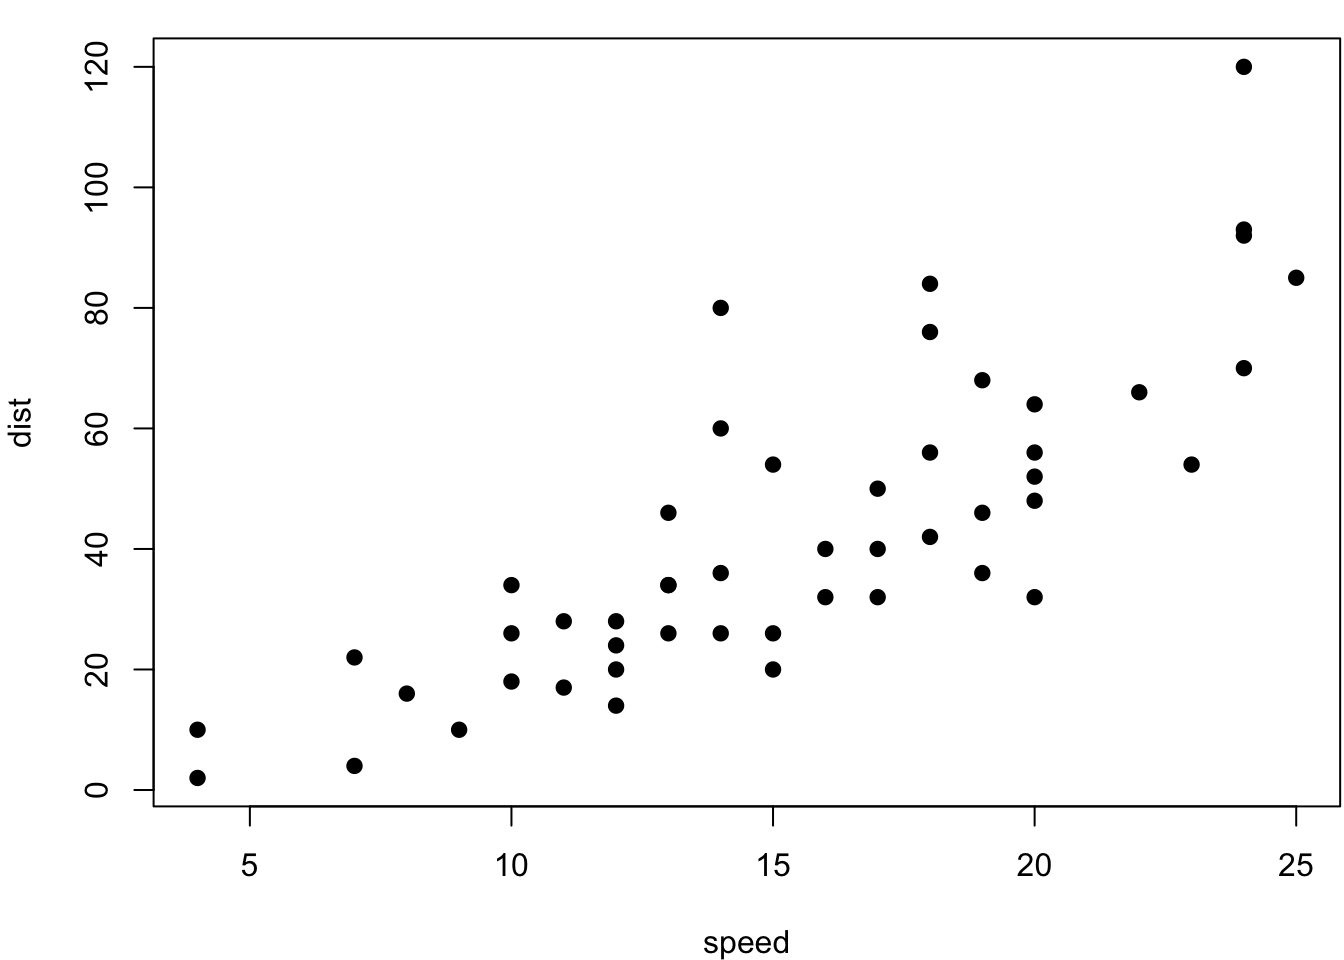
\includegraphics[width=0.9\linewidth]{bookdown_files/figure-latex/hello-1} \caption{雷猴啊,散点图!}\label{fig:hello}
\end{figure}

\begin{Shaded}
\begin{Highlighting}[]
\NormalTok{knitr}\OperatorTok{::}\KeywordTok{kable}\NormalTok{(}
  \KeywordTok{head}\NormalTok{(iris), }\DataTypeTok{caption =} \StringTok{'雷猴啊,iris 数据!'}\NormalTok{,}
  \DataTypeTok{booktabs =} \OtherTok{TRUE}
\NormalTok{)}
\end{Highlighting}
\end{Shaded}

\begin{table}

\caption{\label{tab:iris}雷猴啊,iris 数据!}
\centering
\begin{tabular}[t]{rrrrl}
\toprule
Sepal.Length & Sepal.Width & Petal.Length & Petal.Width & Species\\
\midrule
5.1 & 3.5 & 1.4 & 0.2 & setosa\\
4.9 & 3.0 & 1.4 & 0.2 & setosa\\
4.7 & 3.2 & 1.3 & 0.2 & setosa\\
4.6 & 3.1 & 1.5 & 0.2 & setosa\\
5.0 & 3.6 & 1.4 & 0.2 & setosa\\
5.4 & 3.9 & 1.7 & 0.4 & setosa\\
\bottomrule
\end{tabular}
\end{table}

就这样,你可以一直编下去,直到编不下去。

\hypertarget{wind}{%
\chapter{白苹风末}\label{wind}}

瞎扯几句。

\section{张老爷子}

话说张老爷子写了一首诗:

\begin{quote}
姑苏开遍碧桃时,邂逅河阳女画师。\\
红豆江南留梦影,白苹风末唱秋词。
\end{quote}

\section{彭大将领}

貌似大家都喜欢用白萍风这个意境。又如彭玉麟的对联:

\begin{quote}
凭栏看云影波光,最好是红蓼花疏、白苹秋老;\\
把酒对琼楼玉宇,莫孤负天心月到、水面风来。
\end{quote}

嘿,玛尼玛尼哄。

\cleardoublepage

\hypertarget{appendix-}{%
\appendix \addcontentsline{toc}{chapter}{\appendixname}}


\hypertarget{sound}{%
\chapter{余音绕梁}\label{sound}}

呐,到这里朕的书差不多写完了,但还有几句话要交待,所以开个附录,再啰嗦几句,各位客官稍安勿躁、扶稳坐好。

\bibliography{book.bib,packages.bib}

\backmatter
\printindex

\end{document}
